\chapter{Results}

\section{Deuteron photodisintegraion}
    % \label{sec:deut_bound}

    \begin{figure}[h]
        \begin{center}
        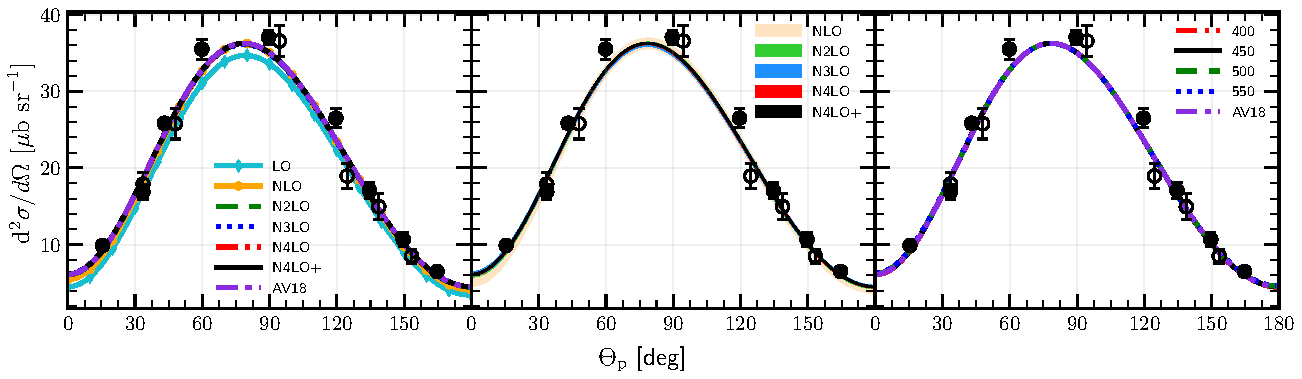
\includegraphics[width=0.95\textwidth]{Figures_python/CROSS2_30mev.pdf}
        \end{center}
        \caption{Differential cross section as a dependence on the outgoing proton angle in the center of mass frame 
        for the photon's energy 30 MeV. Left figure presents results obtained using potential
        with different chiral orders (from LO to N$^4$LO+) with cutoff parameter $\Lambda=450$~MeV
        whereas right figure presents a cutoff dependency and chiral potential N$^4$LO+ was used in all cases.
        For the sake of comparison, predictions obtained with AV18 potential are on both figures as well.}
        \label{CROSS_30}
    \end{figure}
        

    \begin{figure}[h]
        \begin{center}
        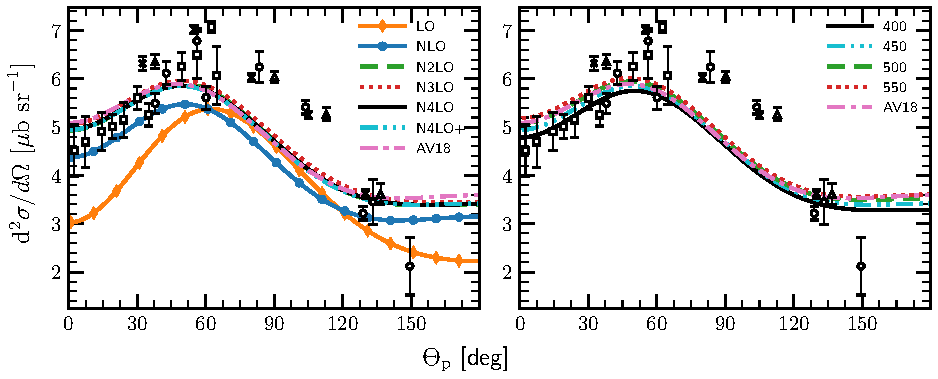
\includegraphics[width=0.95\textwidth]{Figures_python/CROSS2_100mev.pdf}
        \end{center}
        \caption{The same as on the Fig.~\ref{CROSS_30} but for the photon's energy E$_\gamma$=100~MeV}
        \label{CROSS_100}
    \end{figure}

    \begin{figure}[h]
        \begin{center}
        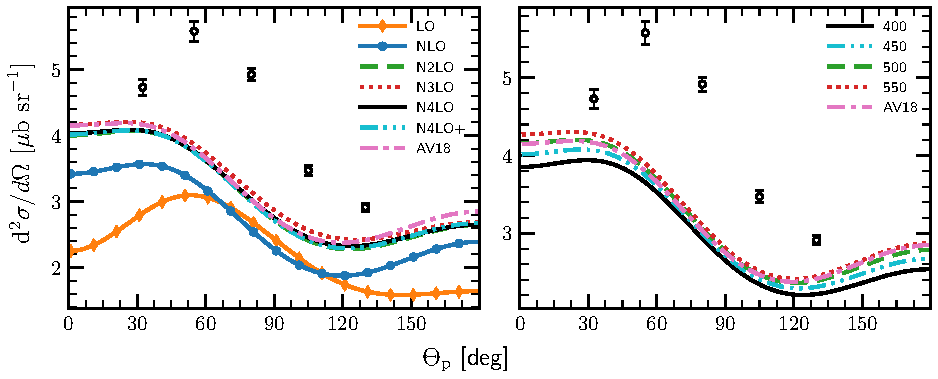
\includegraphics[width=0.95\textwidth]{Figures_python/CROSS2_140mev.pdf}
        \end{center}
        \caption{The same as on the Fig.~\ref{CROSS_30} but for the photon's energy E$_\gamma$=140~MeV}
        \label{CROSS_140}
    \end{figure}
        